\documentclass[aspectratio=169]{beamer}
\usepackage{tikz}

\usepackage{amsthm}
\newtheorem{dfn}[theorem]{Définition}

\usetheme{CambridgeUS}

%Information to be included in the title page:
\title{Sujet 3 – Mise en place d’un module autonome}
\date{Vendredi 17 Juin 2022}

\author[Mise en place d'un module autonome]{Sabrina AKNIOU \\ Anne-Lise FLEISCH \\ Ghassen HNID \\ Bernard NGUYEN}


\usecolortheme{beaver}

\definecolor{bostonuniversityred}{rgb}{0.8, 0.0, 0.0}

\newcommand\padding[2][-3em]{%
\makebox[\linewidth][c]{%
  \begin{minipage}{\dimexpr\textwidth+#1\relax}
  \raggedright#2
  \end{minipage}%
  }%
}


\definecolor{antiquefuchsia}{rgb}{0.57, 0.36, 0.51}
\definecolor{caribbeangreen}{rgb}{0.0, 0.8, 0.6}

\definecolor{Gold}{RGB}{218,165,32}

%Defined Colour Theme and List Sizing
\setbeamercolor{structure}{fg = bostonuniversityred}
\setbeamertemplate{navigation symbols}{}
\setbeamertemplate{headline}{}

\makeatletter
\defbeamertemplate*{footline}{Dan P theme}
{
  \leavevmode%
  \hbox{%
  \begin{beamercolorbox}[wd=.7\paperwidth,ht=2.25ex,dp=1ex,center]{author in head/foot}%
    \usebeamerfont{author in head/foot}\insertshortauthor\expandafter\beamer@ifempty\expandafter{\beamer@shortinstitute}{}{~~(\insertshortinstitute)}
  \end{beamercolorbox}%
  \begin{beamercolorbox}[wd=.3\paperwidth,ht=2.25ex,dp=1ex,center]{date in head/foot}%
    \usebeamerfont{date in head/foot}\insertshortdate{}

  \end{beamercolorbox}}%

}
\makeatother


\begin{document}

% Page de présentation 
\frame{\titlepage}


% 
\begin{frame}

\frametitle{Qu'est ce que le risque inhérent ?}

\padding{
\begin{Large}
\begin{dfn}
Risque extérieur à une entreprise sur lequel elle n’a pas de contrôle et qui affecte les relations d’un partenariat
\end{dfn}
\end{Large}
}

\end{frame}

%
\begin{frame}

\frametitle{Gestion de projet}

\begin{center}
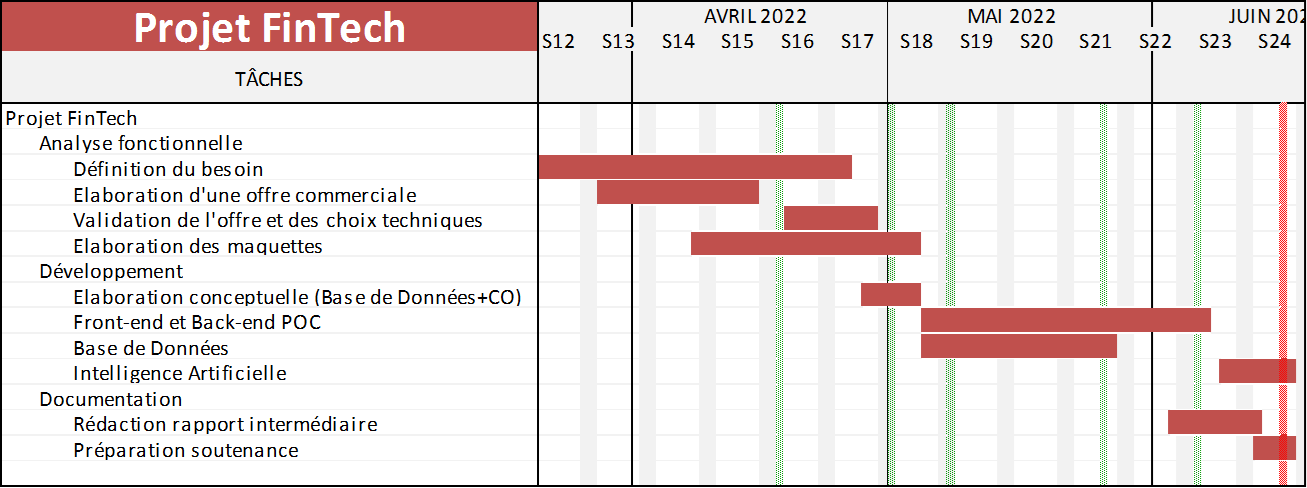
\includegraphics[scale=0.43]{image/gantt}
\end{center}

\end{frame}



%
\begin{frame}

\frametitle{Analyse fonctionnelle}

\padding{
\begin{Large}
\begin{enumerate}
\item[$\rightarrow$] Étapes relatives à l'élaboration du questionnaire
\item[$\rightarrow$] Collection de données
\end{enumerate}
\end{Large}
}

\end{frame}

%
\begin{frame}

\frametitle{Les catégories}

\padding{
\begin{Large}
\begin{enumerate}
\item[$\rightarrow$] Sectorial
\item[$\rightarrow$] Operating
\item[$\rightarrow$] Regulatory
\item[$\rightarrow$] Reputational
\item[$\rightarrow$] Miscellaneous
\end{enumerate}
\end{Large}
}

\end{frame}


%
\begin{frame}

\frametitle{Le formulaire}

\begin{center}
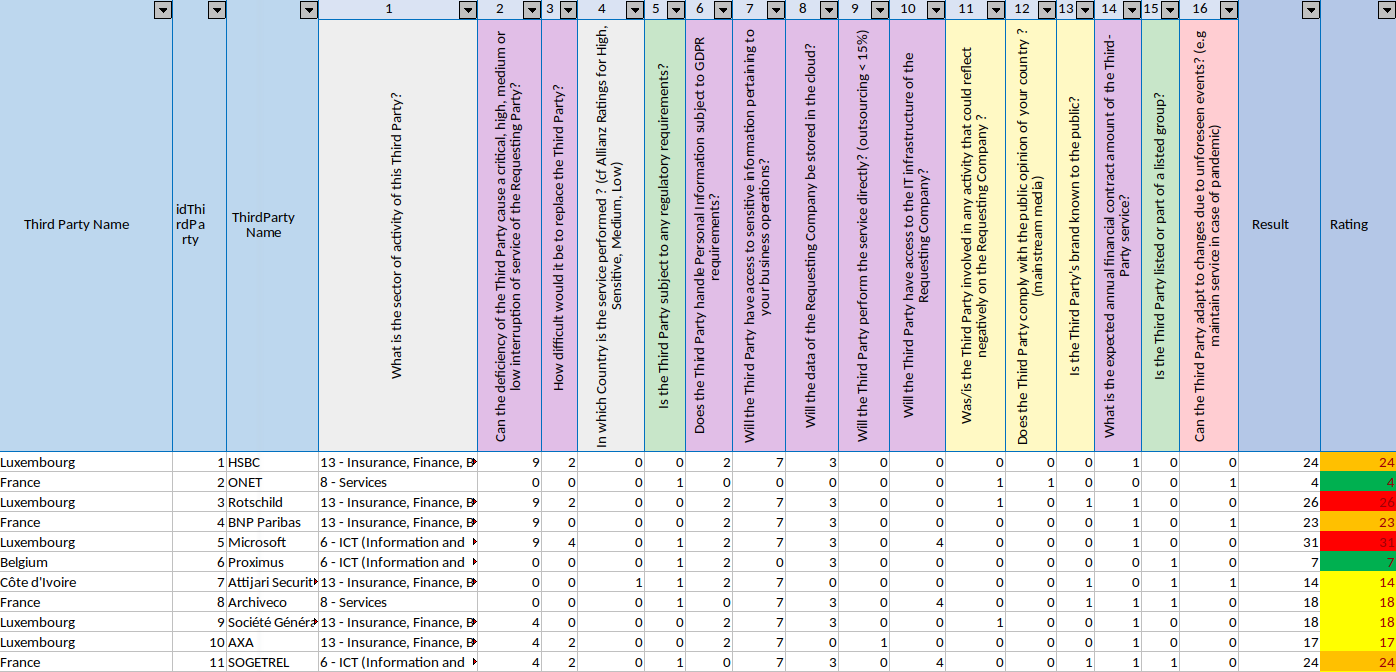
\includegraphics[scale=0.285]{image/excel}
\end{center}

\end{frame}

%
\begin{frame}

\frametitle{Analyse technique}

\padding{
\begin{Large}
\begin{enumerate}
\item[$\rightarrow$] Élaboration conceptuelle
\item[$\rightarrow$] Base de données
\end{enumerate}
\end{Large}
}

\end{frame}



%
\begin{frame}

\frametitle{Élaboration conceptuelle}

\padding{
\begin{Large}
\begin{enumerate}
\item[$\rightarrow$] Réalisation d'un diagramme UML
\end{enumerate}
\end{Large}
}

\end{frame}

%
\begin{frame}

\begin{center}
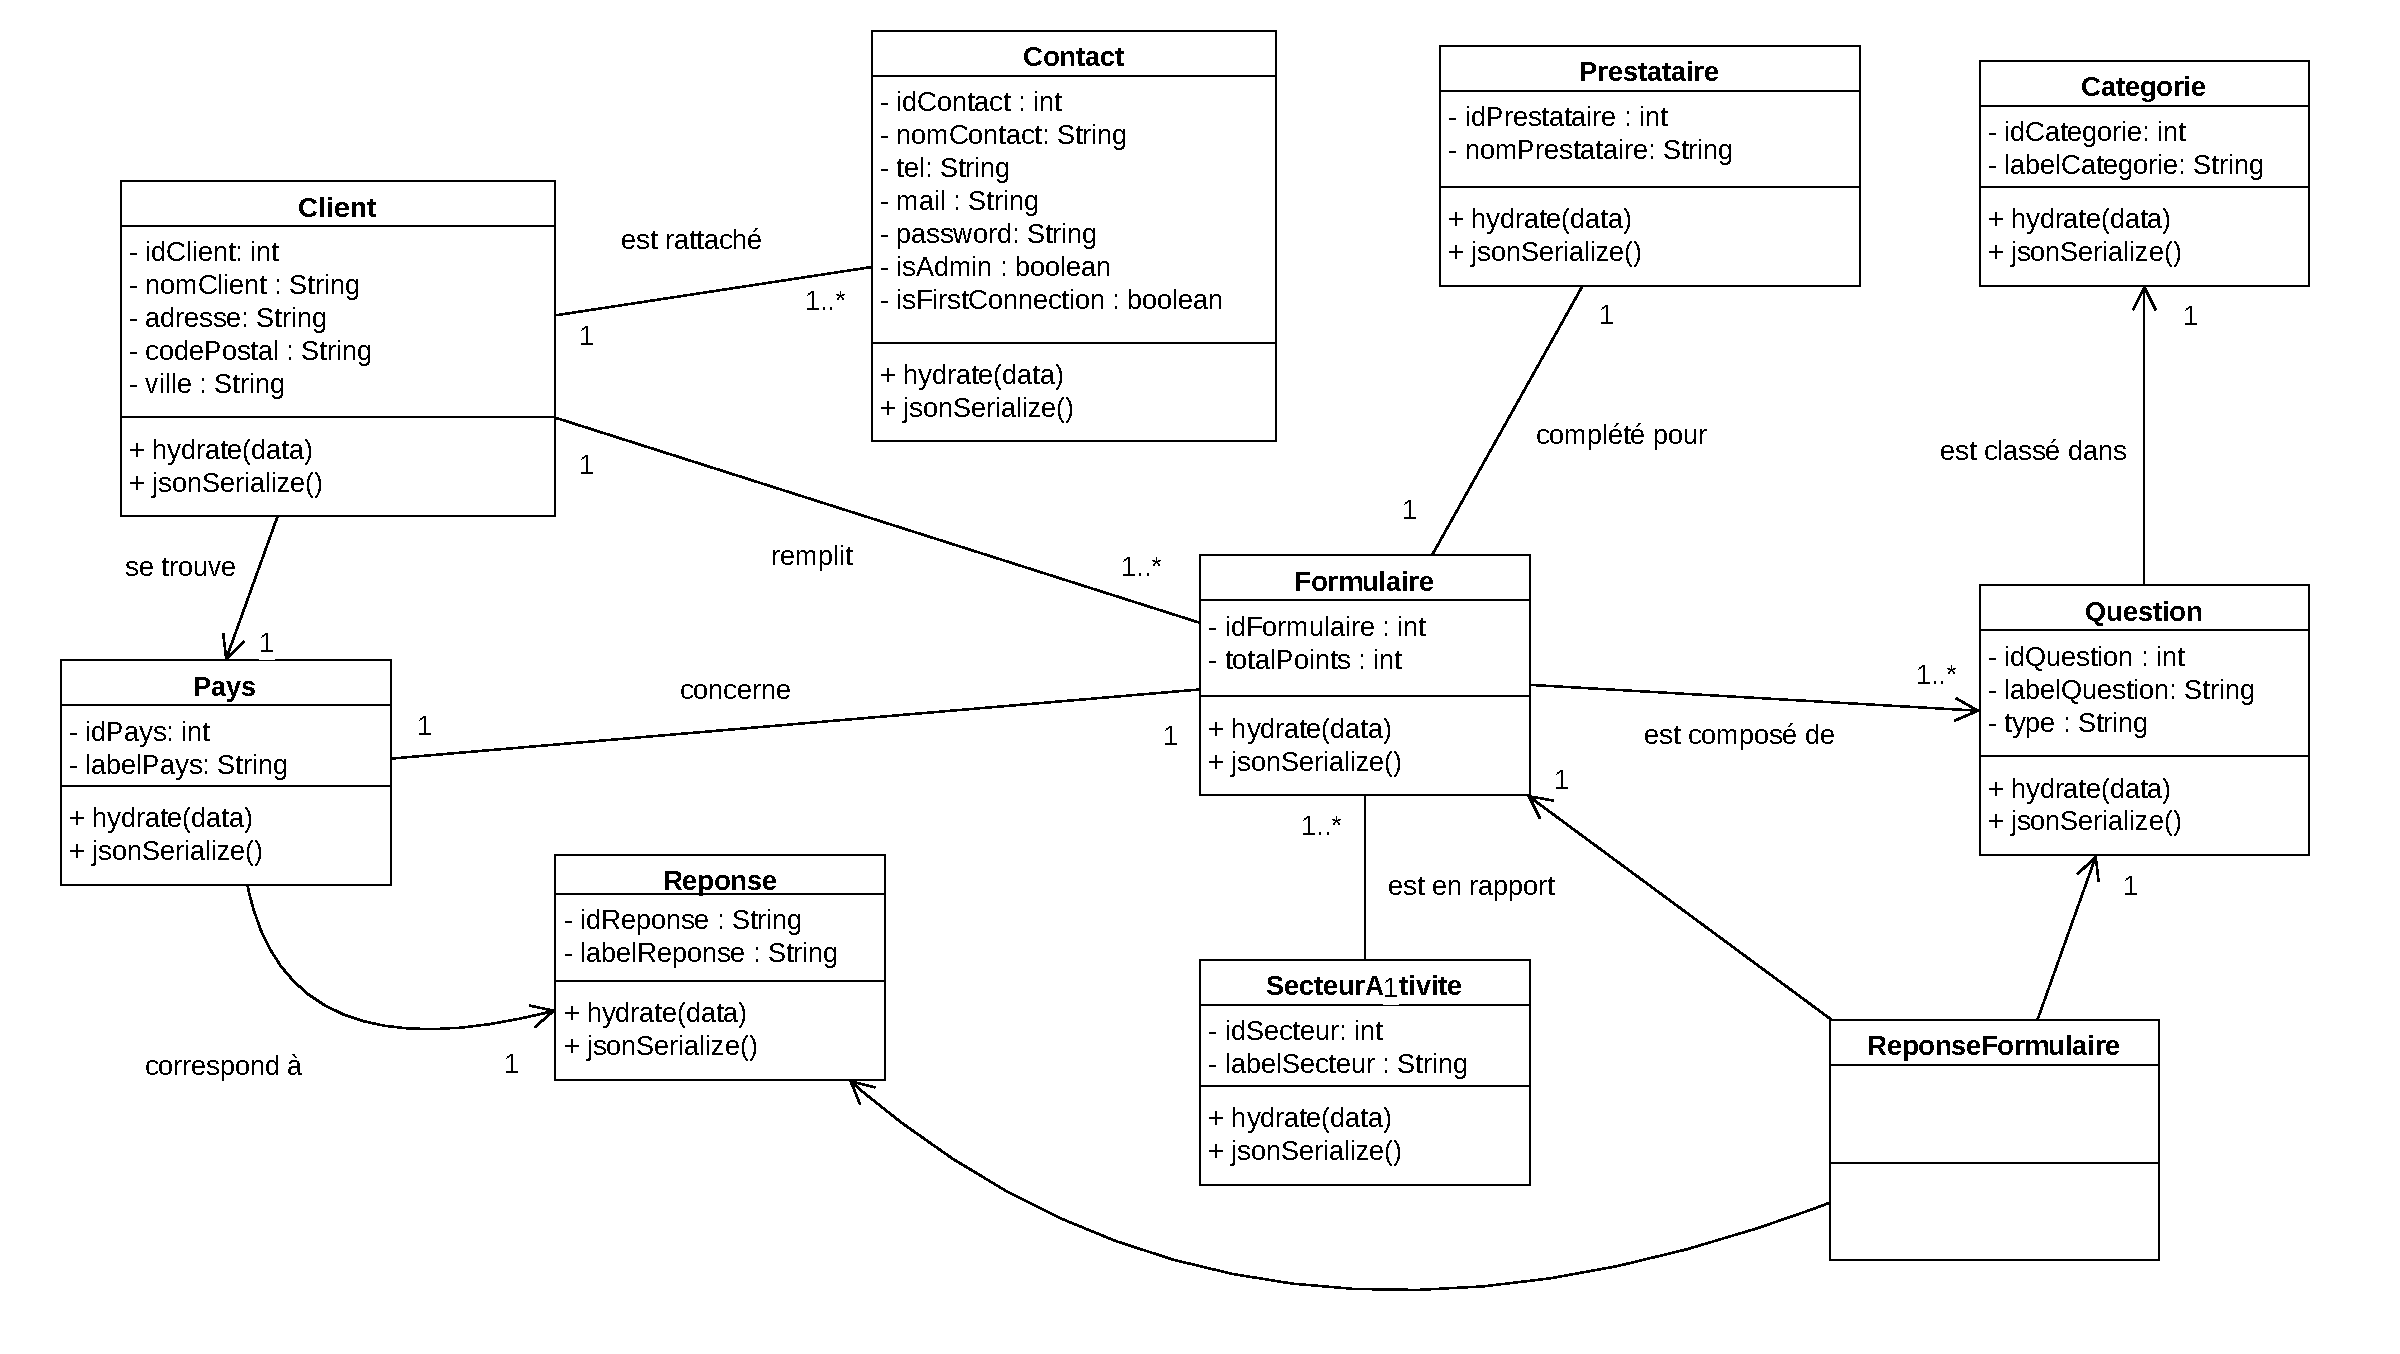
\includegraphics[scale=0.36]{image/uml}
\end{center}

\end{frame}


%
\begin{frame}

\frametitle{Base de données}

\padding{
\begin{Large}
\begin{enumerate}
\item[$\rightarrow$] Schéma relationnel
\item[$\rightarrow$] Schéma E/A
\end{enumerate}
\end{Large}
}
\end{frame}


%
\begin{frame}

\frametitle{Machine Learning : Modèle}

\begin{center}
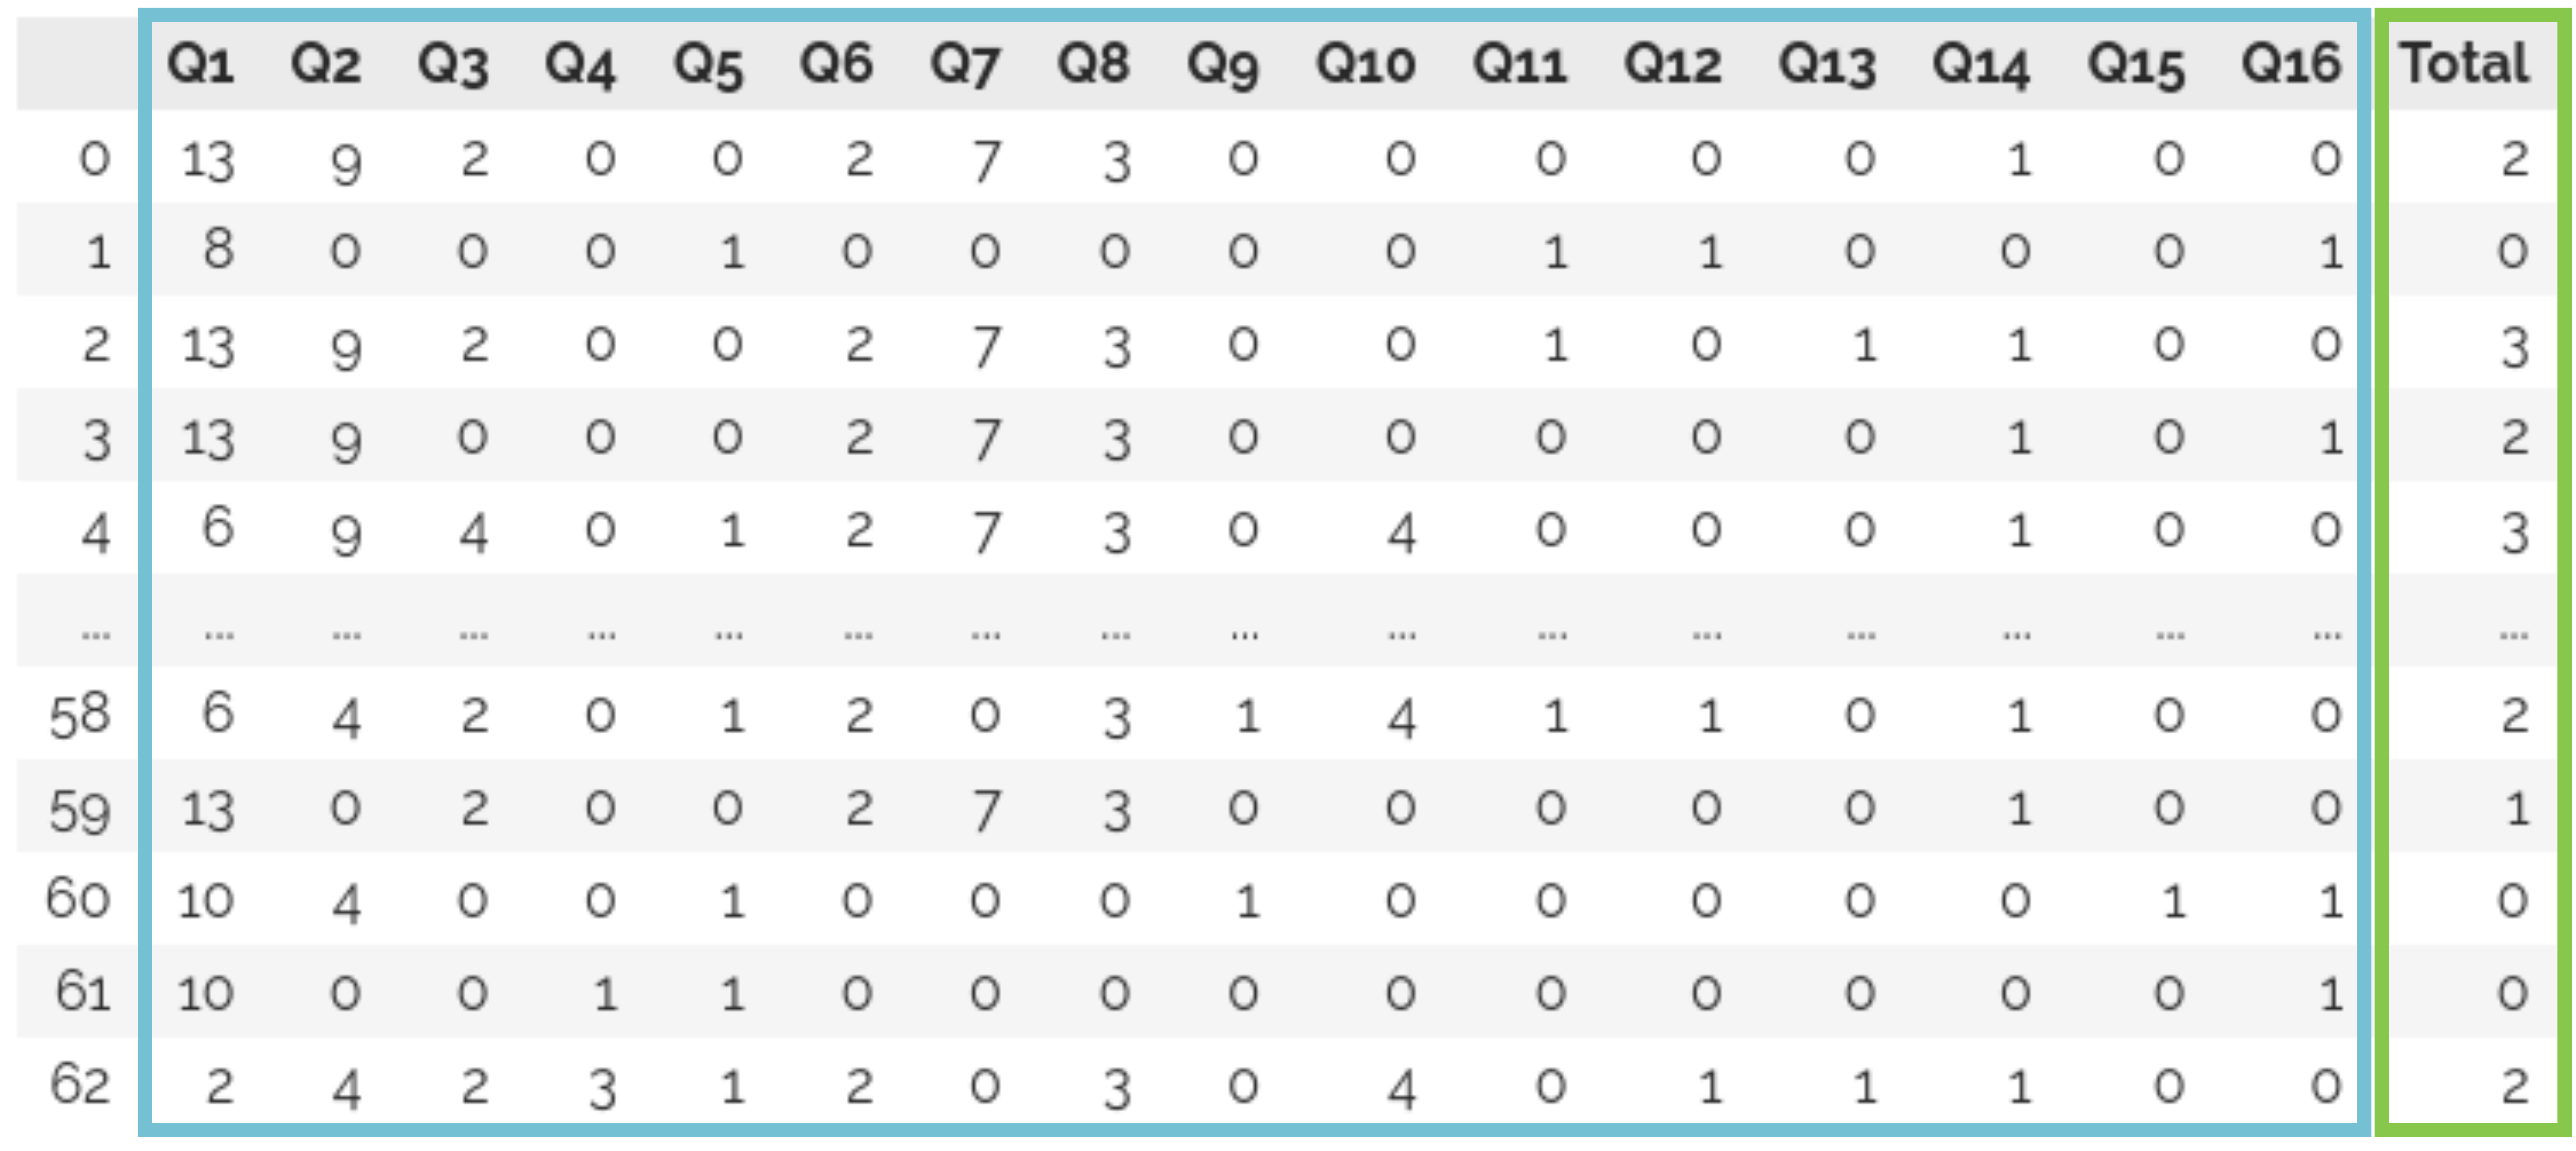
\includegraphics[scale=0.7]{image/mod1}
\end{center}

\end{frame}



%
\begin{frame}

\frametitle{Entraînement et évaluation}

\begin{center}
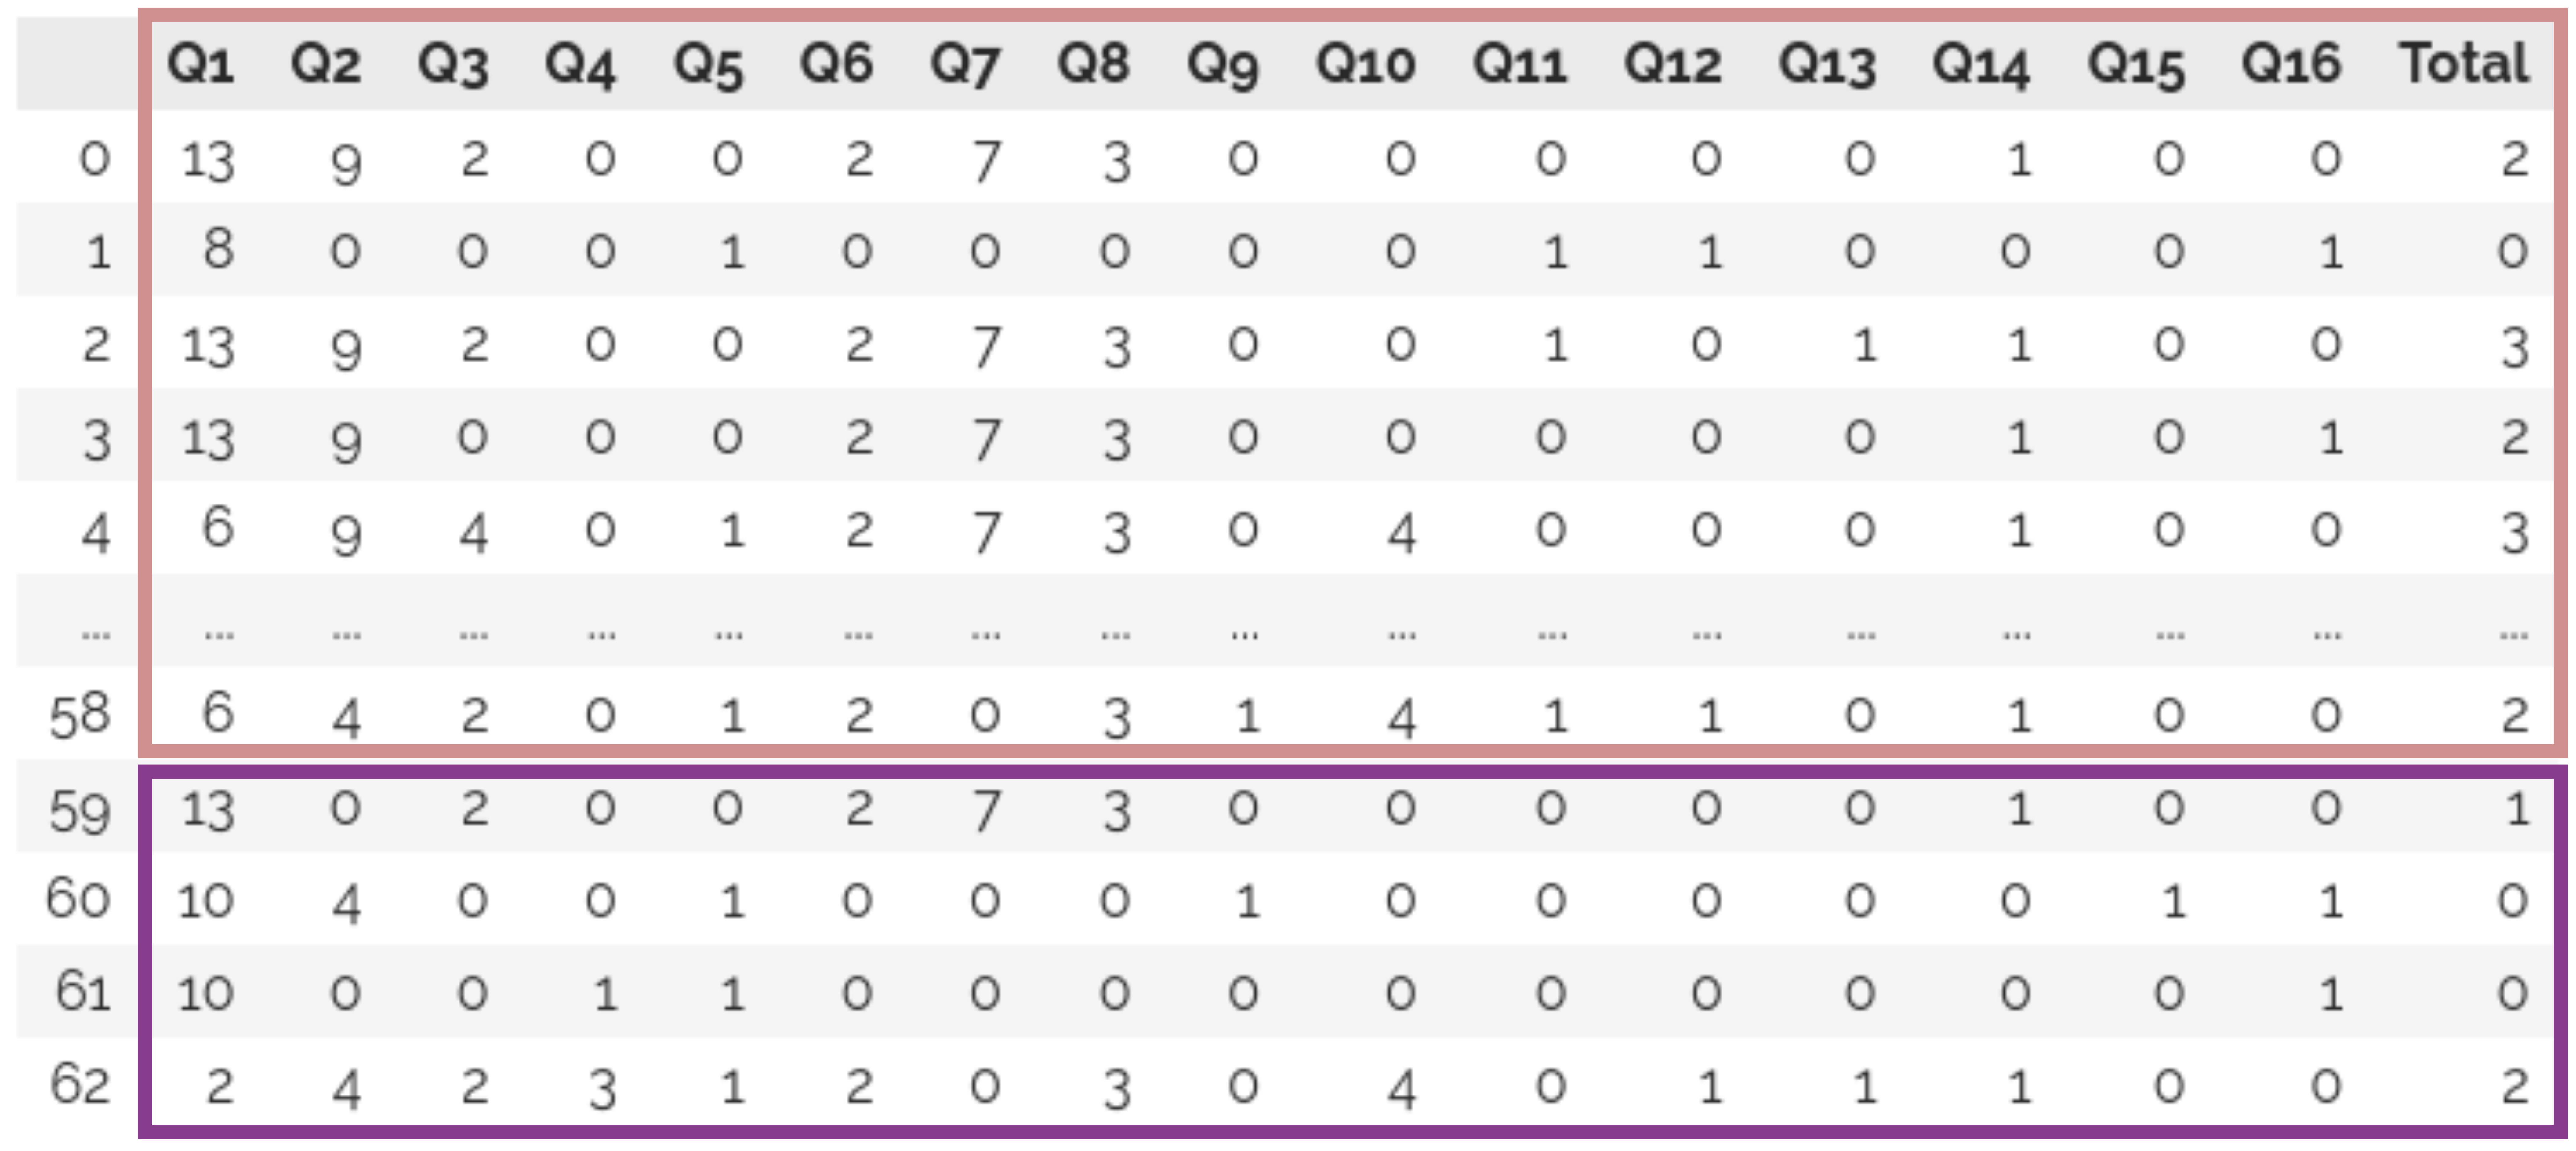
\includegraphics[scale=0.7]{image/mod2}
\end{center}

\end{frame}


%
\begin{frame}

\begin{center}
\includegraphics[scale=0.39]{image/graph-ml}
\end{center}

\end{frame}

%
\begin{frame}

\frametitle{Hypothèses}

\padding{
\begin{Large}
\begin{enumerate}
\item[$\rightarrow$] Sur-entraînement : pas de généralisation
\item[$\rightarrow$] Peu de données cohérentes
\end{enumerate}
\end{Large}
}

\end{frame}



%
\begin{frame}

\padding{
\begin{Huge}
Conclusion...
\end{Huge}
}

\end{frame}


\end{document}